% !TEX root = ../main.tex
\PlanPage{事件入口：固定研究对象的第一步}{吕洪宇}{10}
\noindent\textbf{事件入口的任务，是在分析开始前将研究对象从一句自然语言描述转化为具有时间、方向、来源和版本的结构化记录。}金融研究中的“事件”并非只是一条标题：它需要明确发生或披露的日期、影响对象、方向、材料来源与核验状态，才能在图谱、公司、财务和证据模块中保持同一语义。当前版本因此以已登记事件作为分析入口；研究者选择事件后，前端将事件ID与数据版本提交给总控，而不是把页面文字直接交给后续模块解释。

\begin{center}
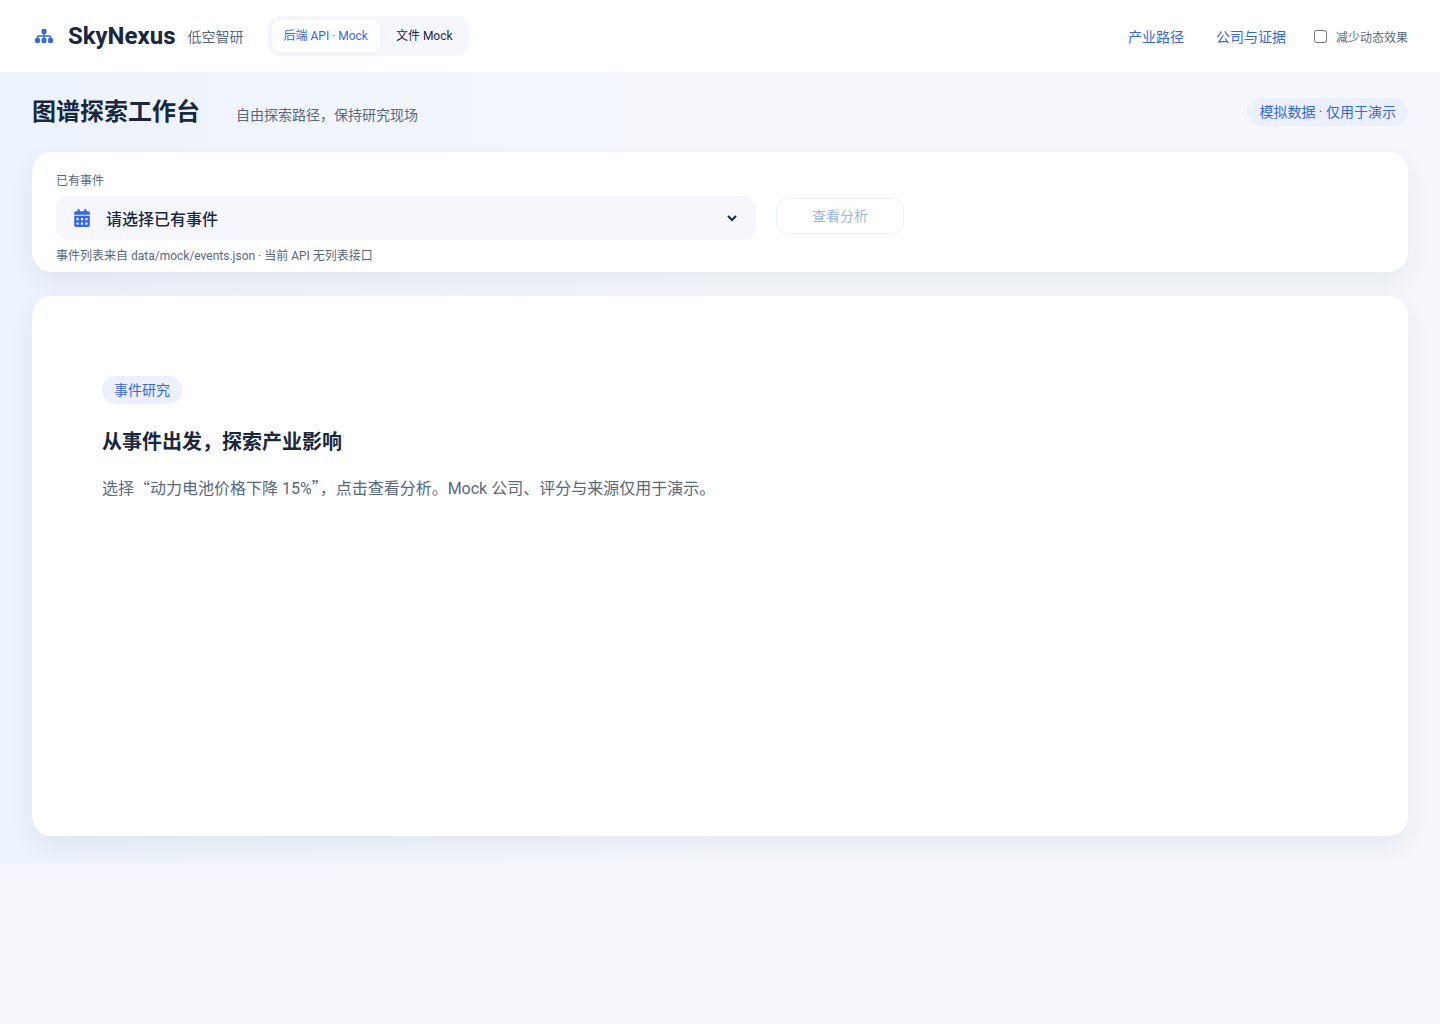
\includegraphics[width=0.88\linewidth,height=0.37\textheight,keepaspectratio]{assets/hongyulyu714-prog/fig-event-entry.png}
\PlanFigureCaption{图10-1}{事件入口截图。工作台展示当前事件选择和分析按钮；截图来源于仓库\texttt{docs/screenshots/01-entry.png}。当前事件池服务于Mock全链路验证，研究者在发起分析前能够确认事件名称与模式。}
\end{center}

对于任何拟接入的事件，系统首先建立事件卡：\texttt{event\_id}承担跨模块主键功能，事件名称与类型定义研究主题，日期与方向限定时间语境和作用方向，受影响节点为图谱查询设定起点，来源标题、URL与核验状态为后续事实审阅保留入口。只有当这些字段随同事件进入总控，报告中的路径、公司、分数和证据才可以被识别为围绕同一个研究对象生成\cite{lhy-contracts,lhy-architecture}。

\begin{center}\small 表10-1\quad 事件对象的字段设计及其在研究链中的作用\par\vspace{1mm}
\begin{tabularx}{\linewidth}{p{0.19\linewidth}p{0.26\linewidth}X}
\toprule
字段组 & 在系统中的作用 & 研究审阅时应回答的问题\\
\midrule
唯一标识 & \texttt{event\_id}连接路径、公司、评分、证据和运行记录 & 这些对象是否确实属于同一事件，而非来自相似但不同的行业新闻？\\
事实描述 & 名称、类型、日期、地区、方向与受影响节点定义研究范围 & 事件究竟改变了什么，变化发生在哪个时间与产业环节？\\
来源信息 & 标题、URL、发布日期、摘录与核验状态保留事实定位 & 研究者能否回到原始材料，确认当前表述没有超出来源？\\
版本信息 & \texttt{data\_version}约束本次运行使用的一组数据资产 & 报告中的路径、评分和证据是否来自可识别且相互兼容的版本？\\
运行信息 & \texttt{run\_id}、开始/结束时间、状态与错误文本记录分析过程 & 同一输入是否可重放；若失败，失败发生在何处？\\
\bottomrule
\end{tabularx}\end{center}

事件被提交后，总控首先登记一次运行，再读取对应版本的五类输入。未知事件、未注册版本或不符合契约的输入会在报告形成前返回可读错误，并写入失败运行记录\cite{lhy-orchestrator}。这条流程使事件识别、数据治理与分析启动成为同一件事：研究对象一旦变化，后续所有推理均以新的事件记录和新运行记录为准。自然语言解析可以在后续作为候选事件发现模块接入，但其输出同样必须经过来源、字段、版本与人工复核后才能进入研究主链。
